\subsection{Teknologianalyse}
\begin{frame}{Teknologianalyse}
    \framesubtitle {BoatCloud}
        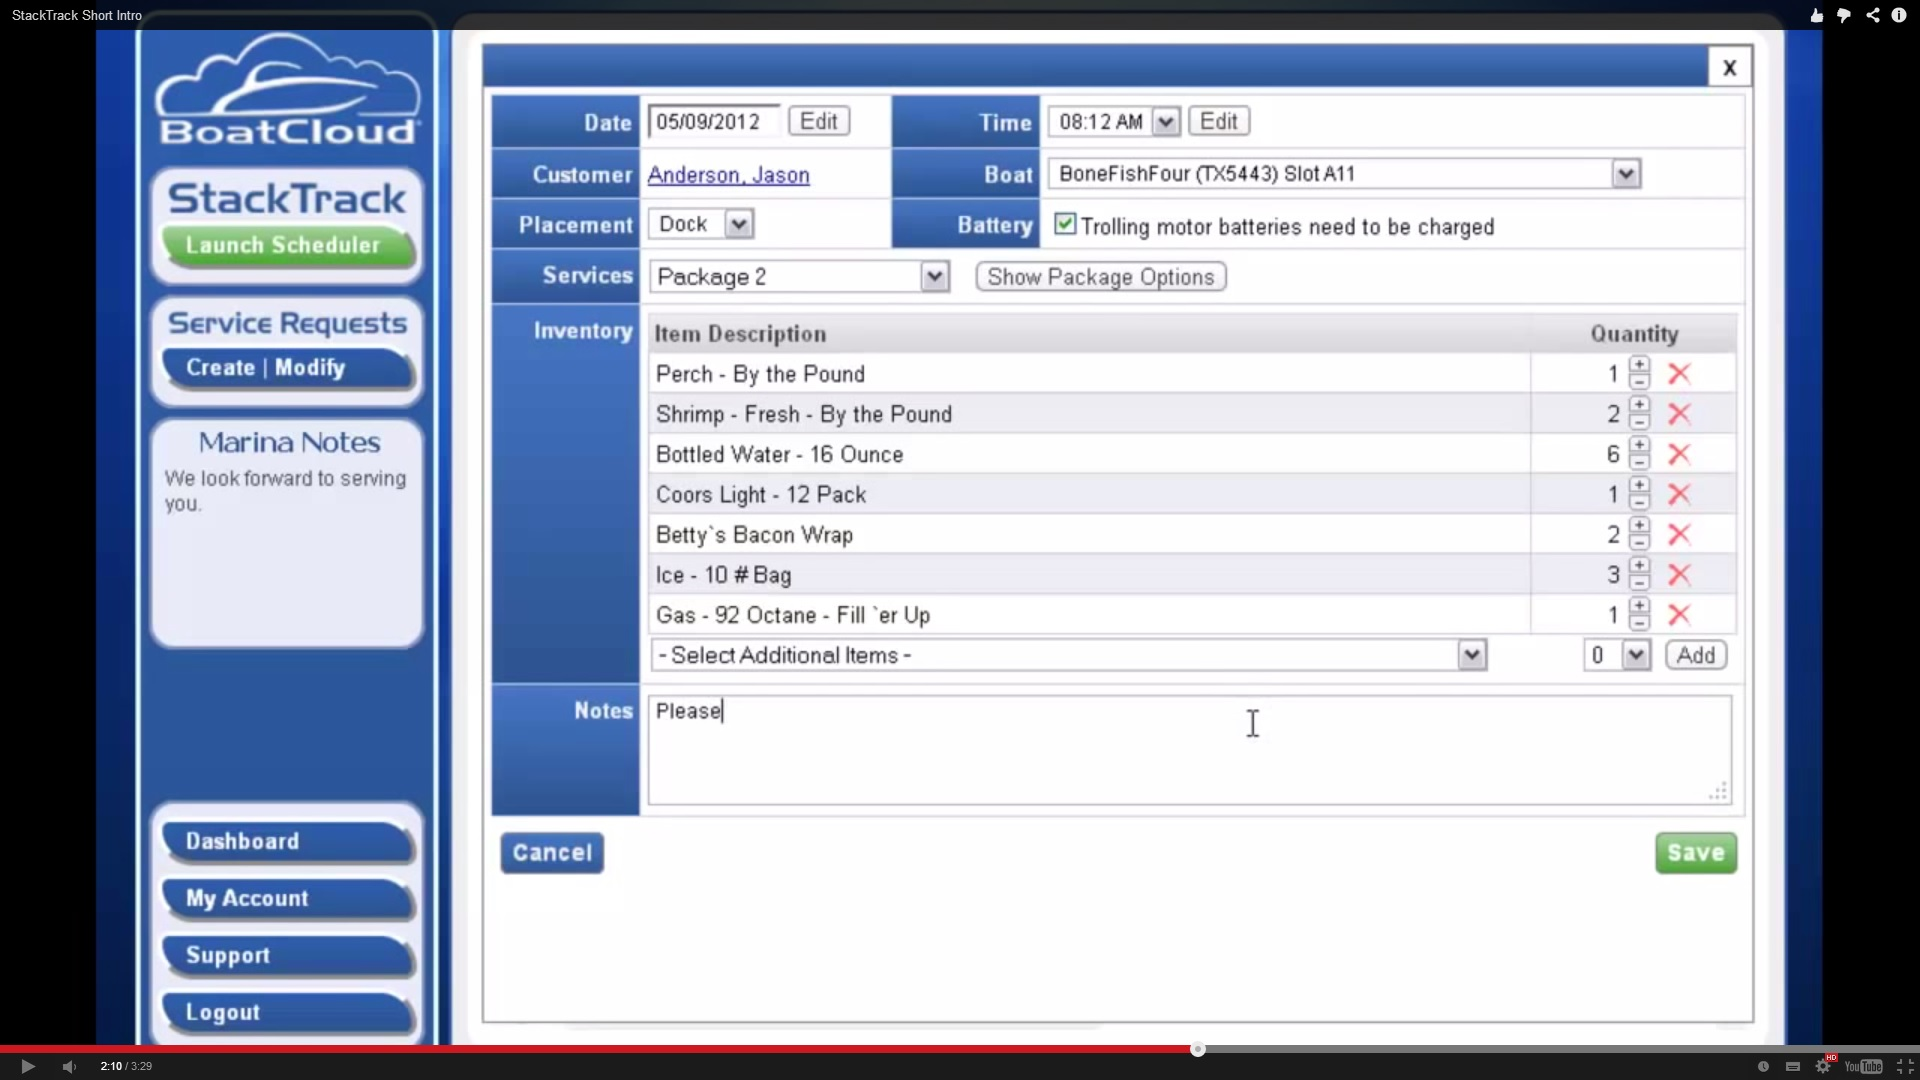
\includegraphics[width=1\textwidth]{images/StackTrack.jpg}
\end{frame}

\begin{frame}{Teknologianalyse}
    \framesubtitle {BoatCloud}
        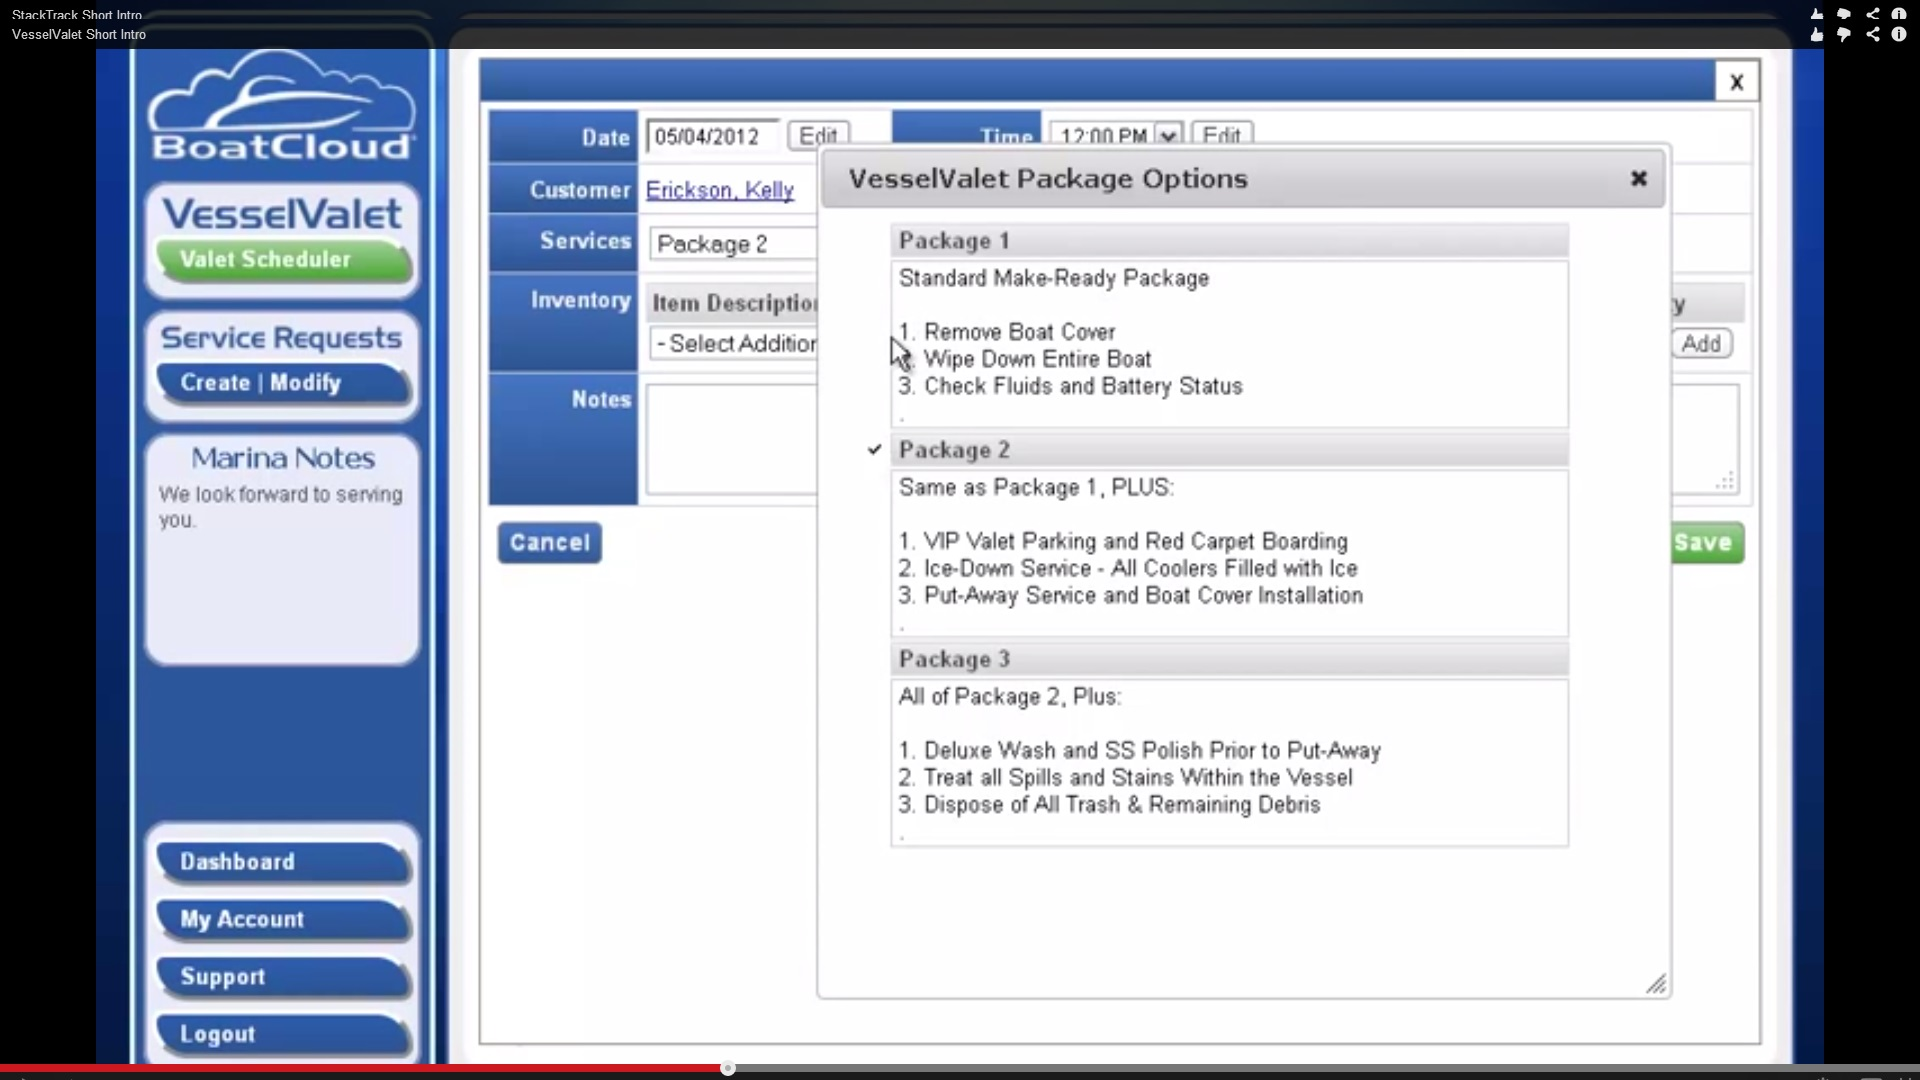
\includegraphics[width=1\textwidth]{images/VesselValet.jpg}  
\end{frame}

\begin{frame}{Teknologianalyse}
    \framesubtitle {BoatCloud}
        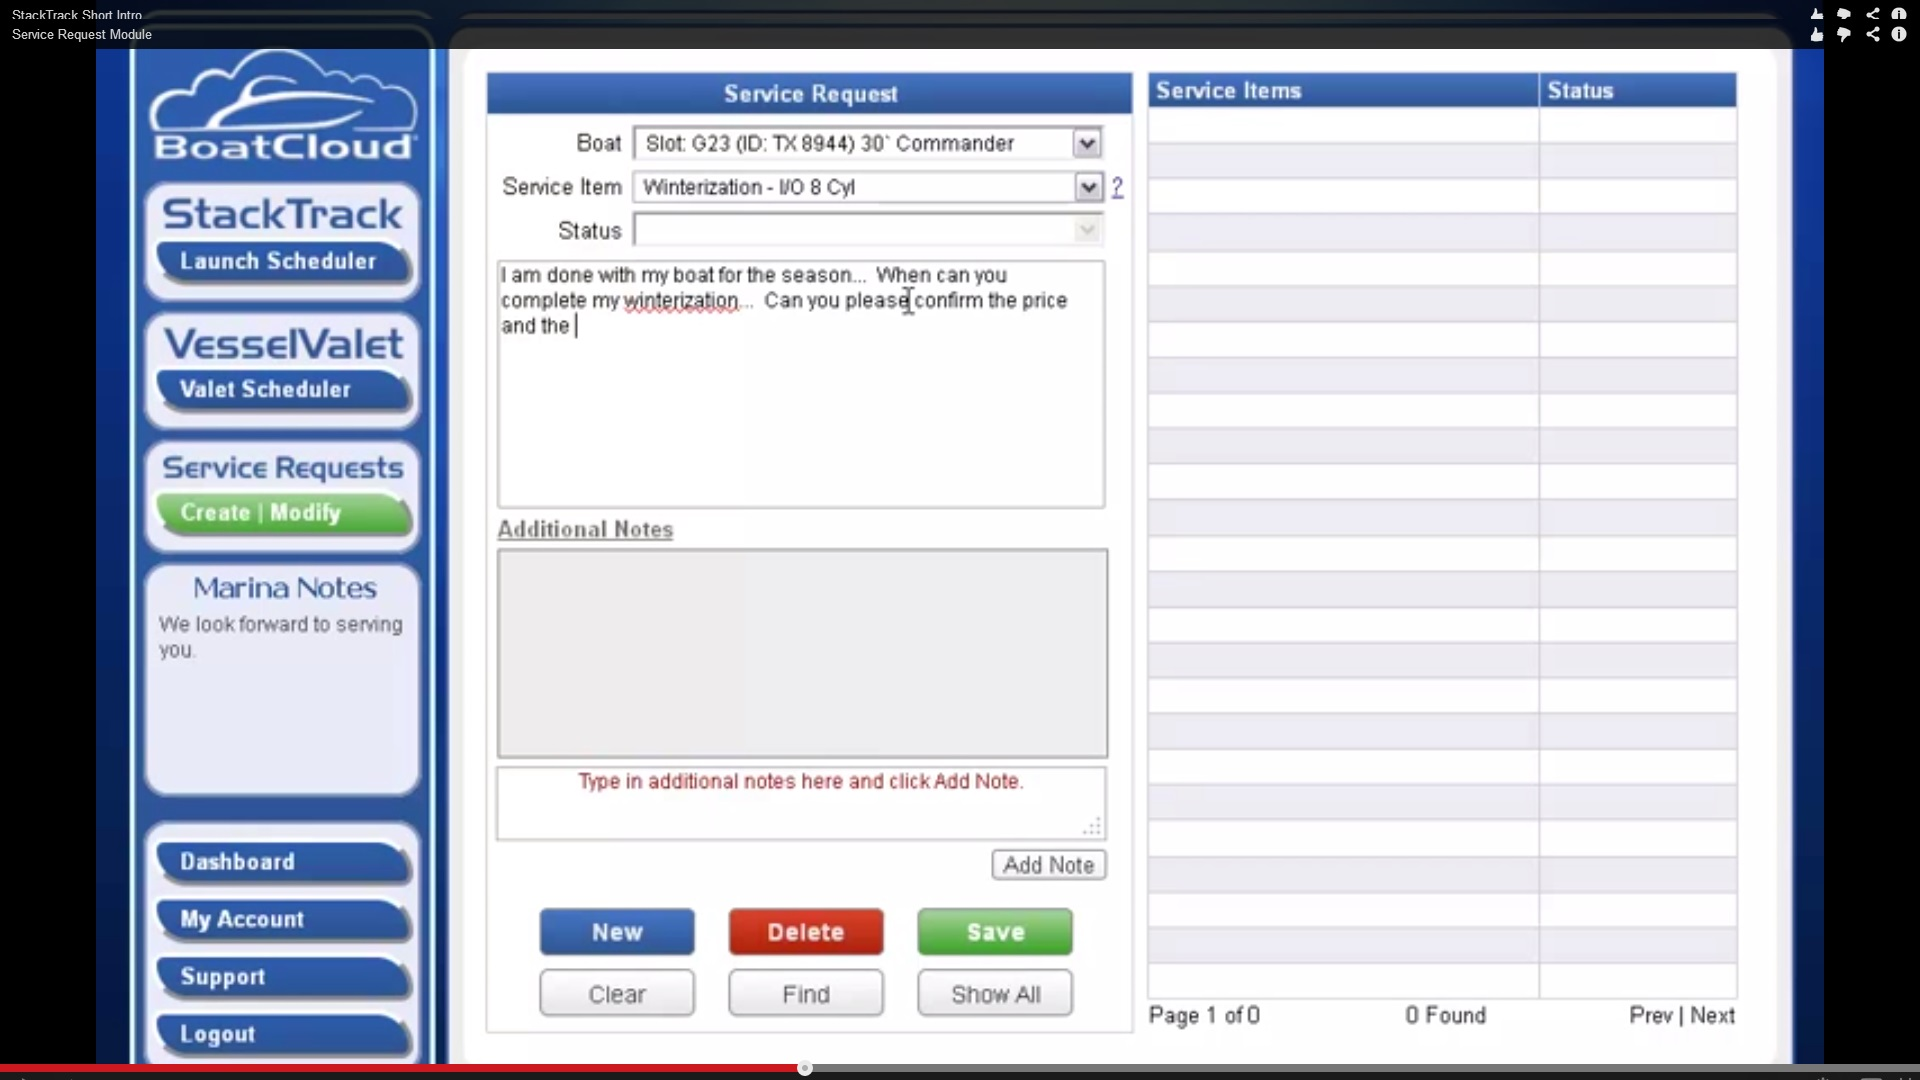
\includegraphics[width=1\textwidth]{images/TicketTracker.jpg} 
\end{frame}

\begin{frame}{Teknologianalyse}
    \framesubtitle {SailingClubManager}
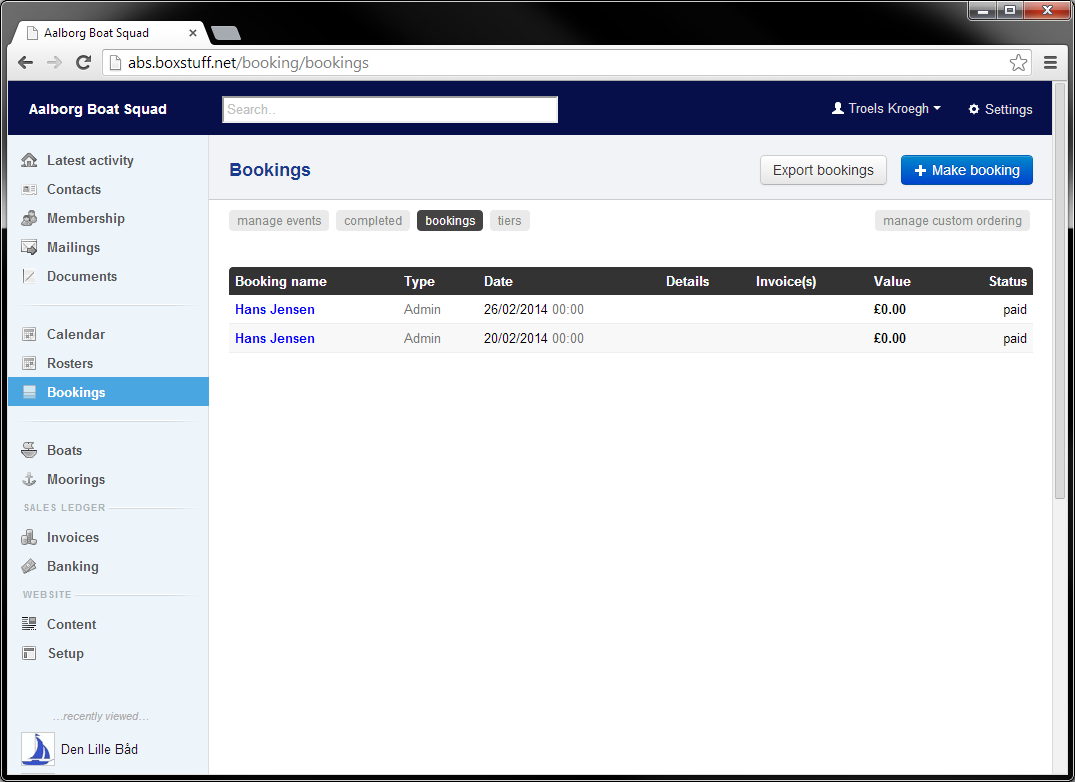
\includegraphics[width=1\textwidth]{images/SCM.png}
\end{frame}

\begin{frame}{Teknologianalyse}
    \framesubtitle {ForeningLet}
        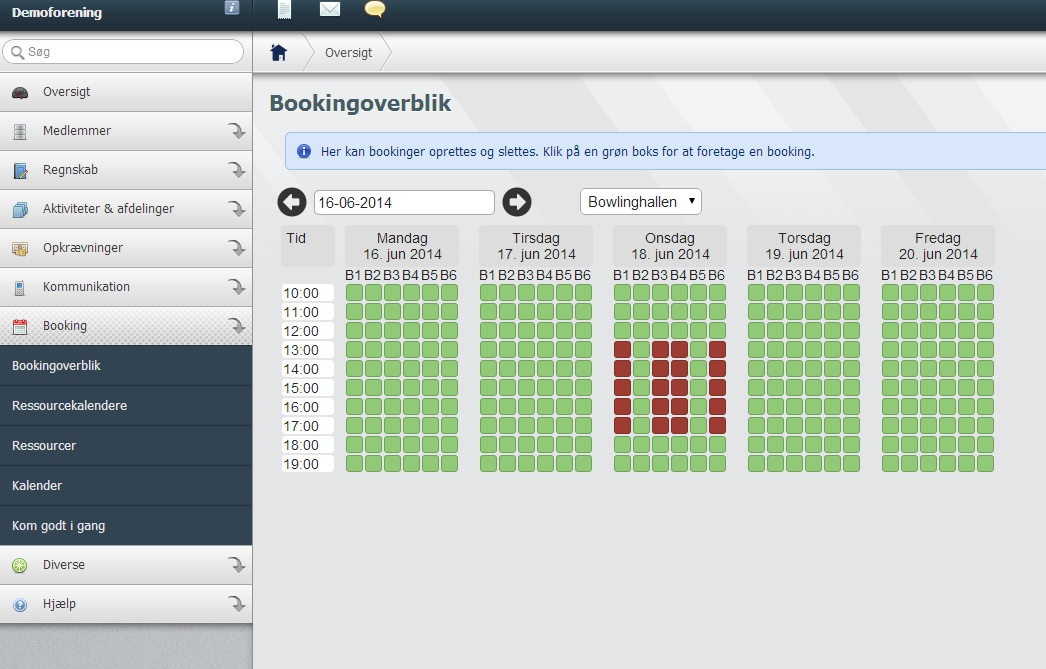
\includegraphics[width=1\textwidth]{images/ForeningLet.jpg}
\end{frame}


\subsection{Problemformulering}

\begin{frame}{Opsummering}
\begin{itemize}
   \item Fritidsklubber
   \item Sundet
   \item ForeningLet
\end{itemize}
\end{frame}

\begin{frame}{Problemformulering}

\begin{beamerboxesrounded}[upper=headerCol,lower=bodyCol,shadow=true]{Problemformulering}
\textit{Det er et problem at frivillige i fritidsklubber med specielle udlejningsmuligheder, så som Sejlklubben Sundet, benytter unødvendig arbejdskraft på fysisk dokumenthåndtering vedrørende udlånte faciliteter, undervisning og begivenhedsorganisation. Hvordan kan der udvikles et system som kan hjælpe med at danne overblik over sådanne opgaver?}
\end{beamerboxesrounded}

  \begin{itemize}
      
    \item Hvilke informationer ville et sådan system skulle holde styr på?
    \item Er det muligt at arbejde sammen med systemer allerede I brug ved klubben?
    \item Hvordan skal et sådan system arrangeres for at gøre det let at bruge?
  \end{itemize}
\end{frame}